\begin{frame}{$d(K^-, n \pi)"\Sigma"$ Fitting (MC shifted)}
  \begin{tabular}{cc}
    \begin{minipage}{0.5\hsize}
      \begin{figure}
        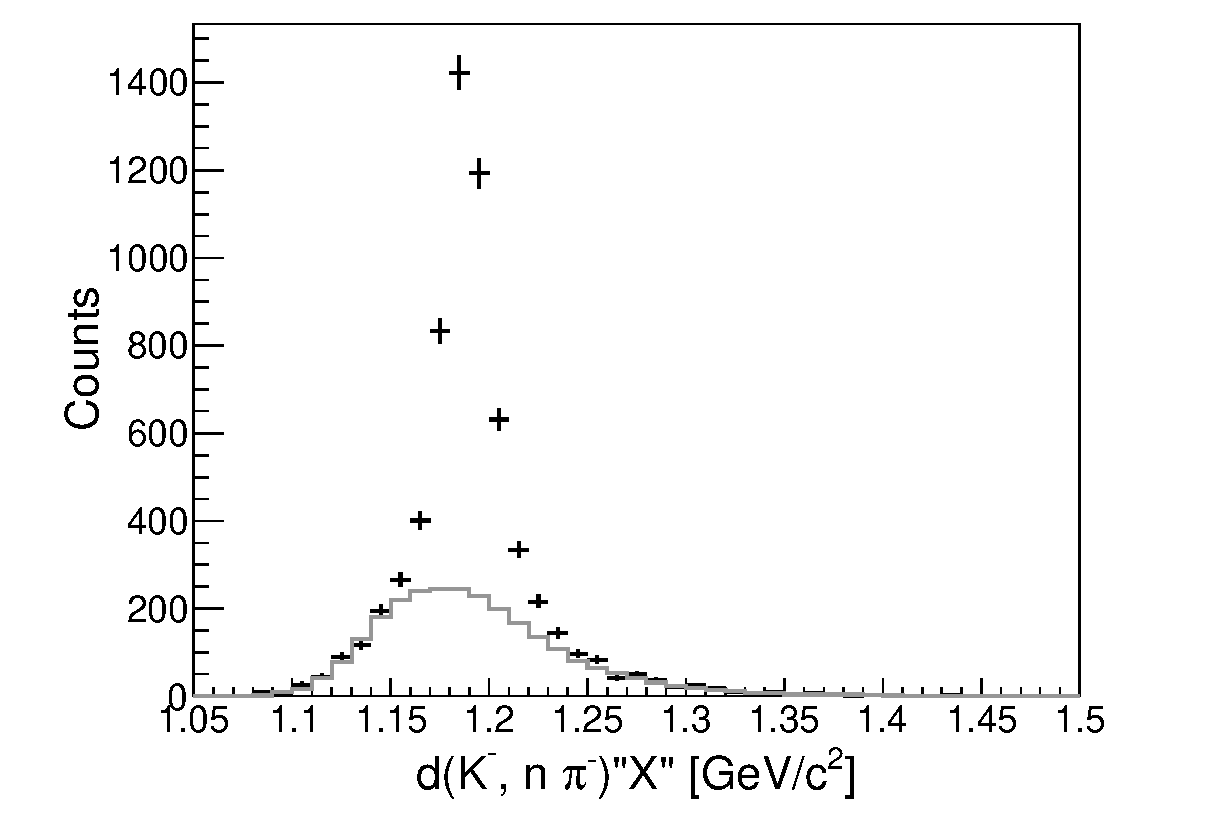
\includegraphics[width=3cm]{../pic/Run78/KN_ana_old2/fitKNpim_MM_data_wBG.eps}
      \end{figure}
    \end{minipage}

    \begin{minipage}{0.5\hsize}
      \begin{figure}
        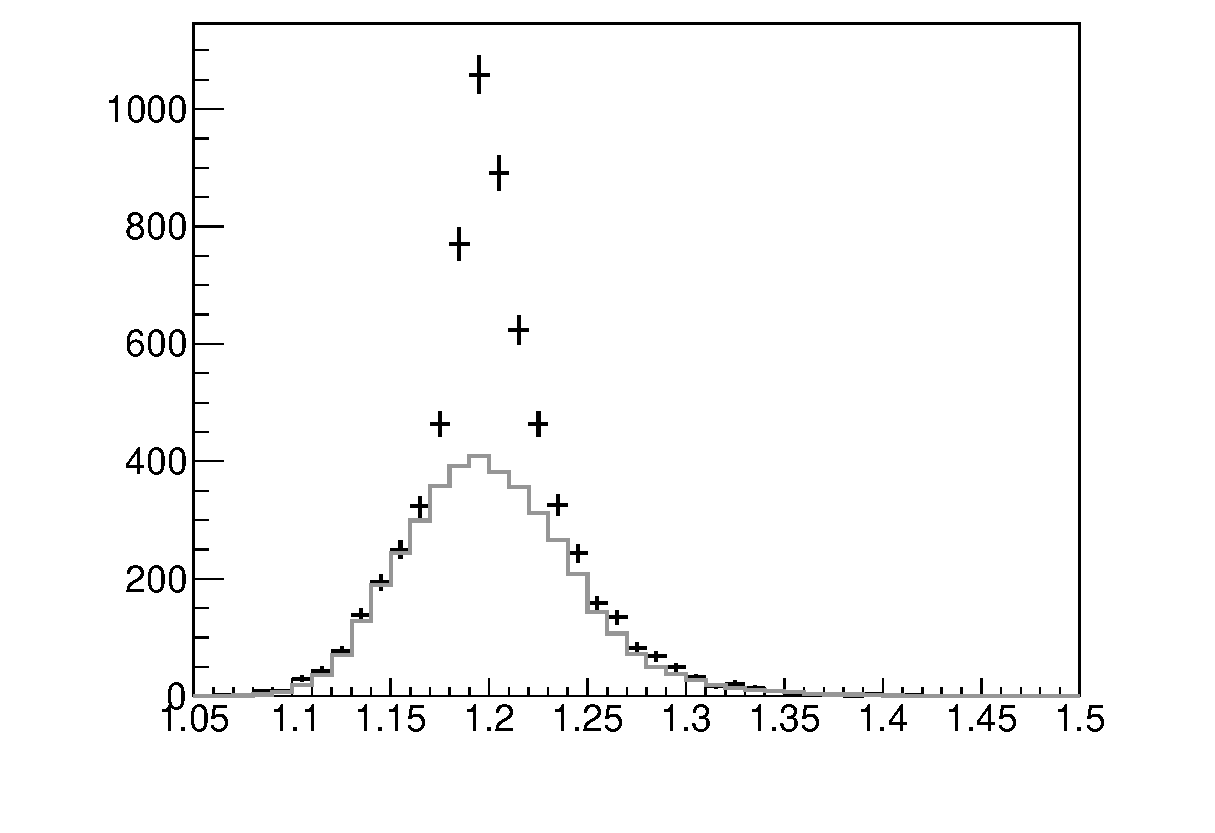
\includegraphics[width=3cm]{../pic/Run78/KN_ana_old2/fitKNpip_MM_data_wBG.eps}
      \end{figure}
    \end{minipage}
  \end{tabular}

  \begin{tabular}{cc}
    \begin{minipage}{0.5\hsize}
      \begin{figure}
        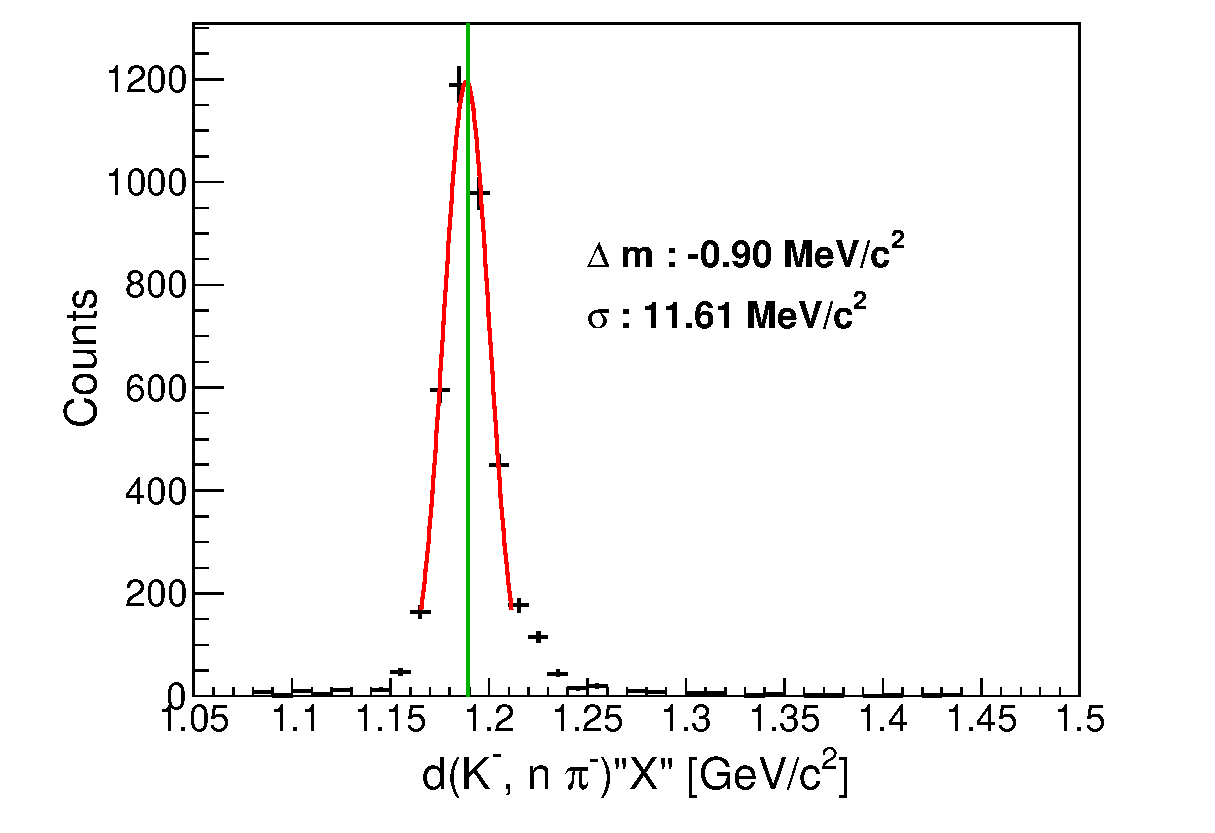
\includegraphics[width=3cm]{../pic/Run78/KN_ana_old2/fitKNpim_MM_data.eps}
      \end{figure}
    \end{minipage}

    \begin{minipage}{0.5\hsize}
      \begin{figure}
        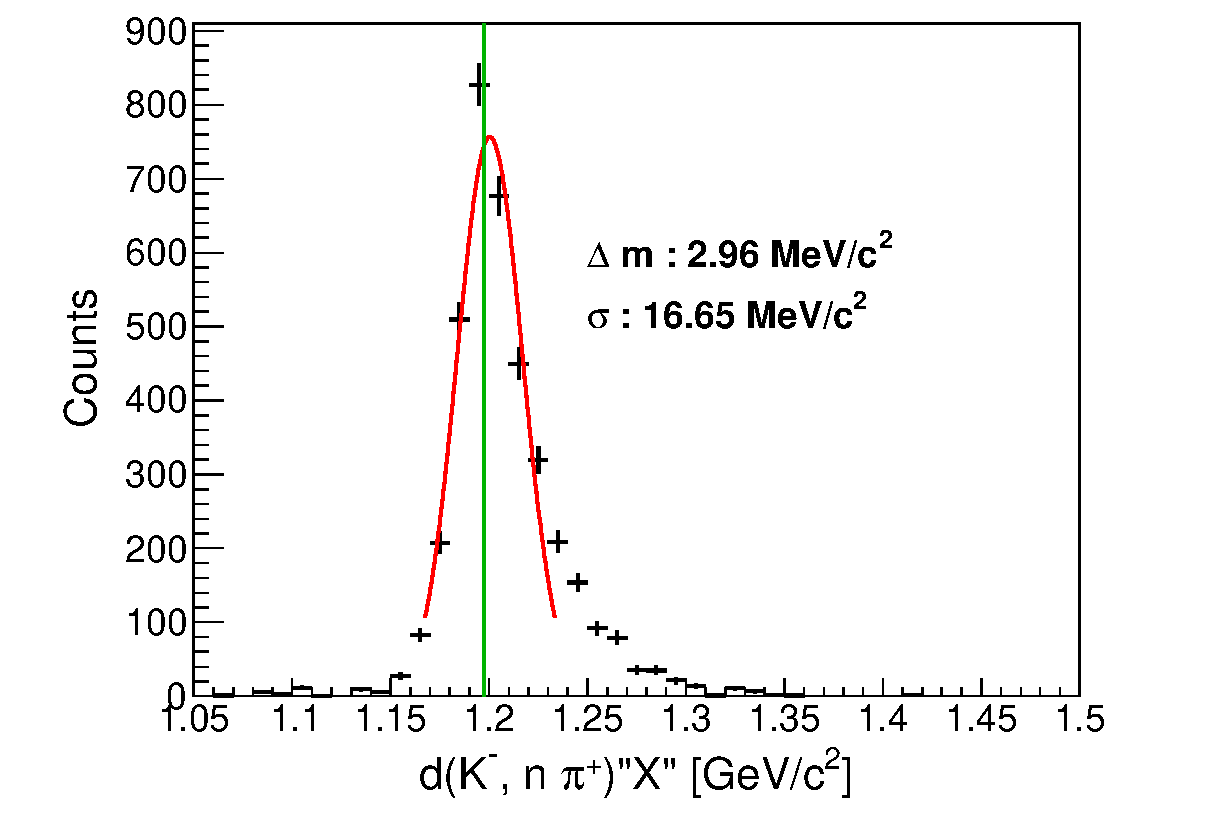
\includegraphics[width=3cm]{../pic/Run78/KN_ana_old2/fitKNpip_MM_data.eps}
      \end{figure}
    \end{minipage}
  \end{tabular}

  \begin{tabular}{cc}
    \begin{minipage}{0.5\hsize}
      \begin{figure}
        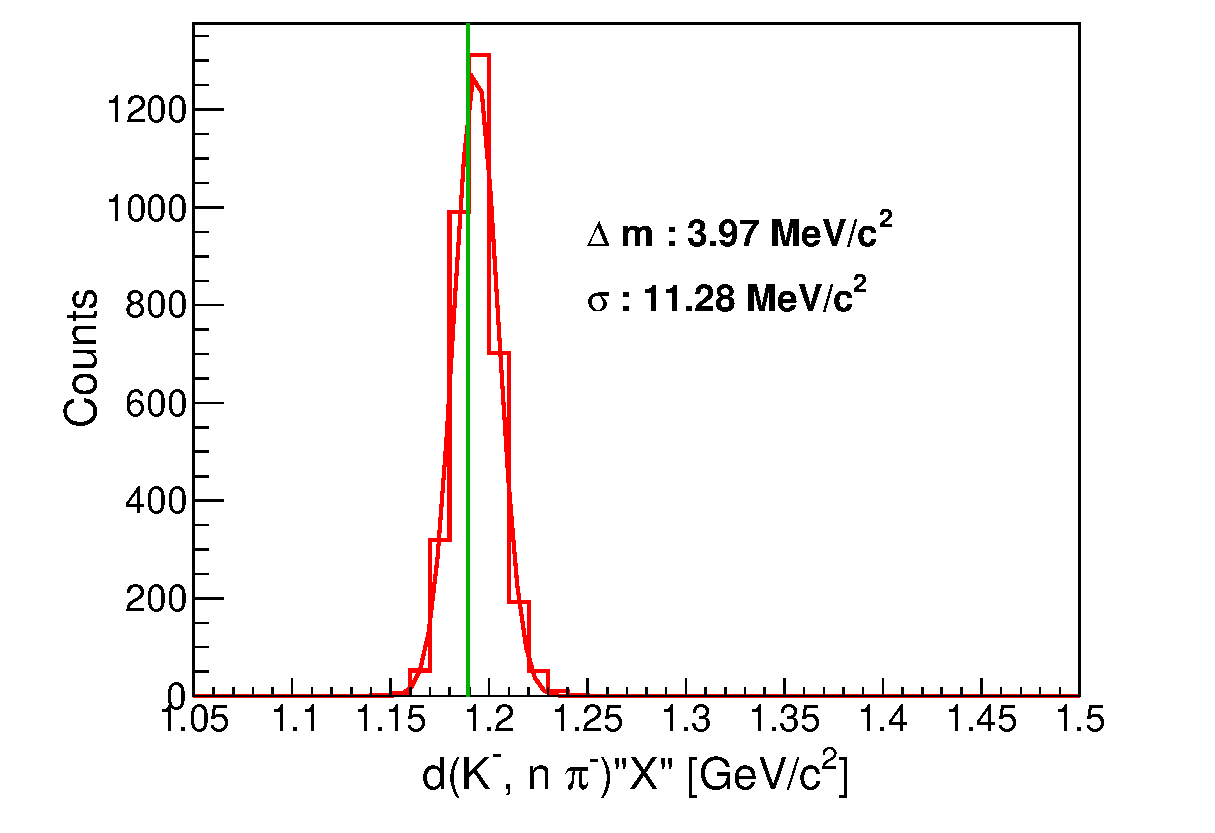
\includegraphics[width=3cm]{../pic/Run78/KN_ana_old2/fitKNpim_MM_MC.eps}
      \end{figure}
    \end{minipage}

    \begin{minipage}{0.5\hsize}
      \begin{figure}
        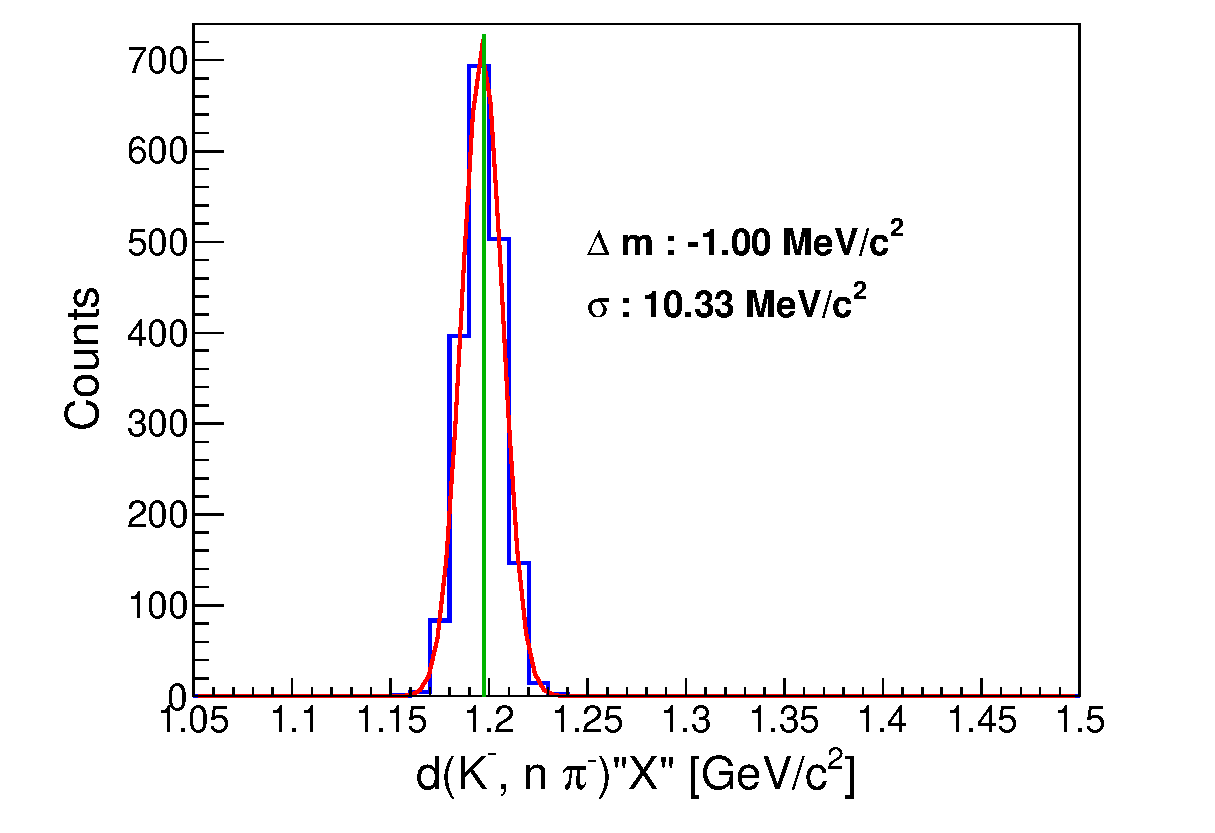
\includegraphics[width=3cm]{../pic/Run78/KN_ana_old2/fitKNpip_MM_MC.eps}
      \end{figure}
    \end{minipage}
  \end{tabular}
\end{frame}
